% begin module trig-functions-example2
\begin{frame}
\begin{example}
If $\cos \theta = \frac{2}{5}$ and $0 < \theta < \pi /2$, find the other five trigonometric functions of $\theta$.
\begin{columns}[c]
\column{.3\textwidth}
\ \only<handout:0| -1>{%
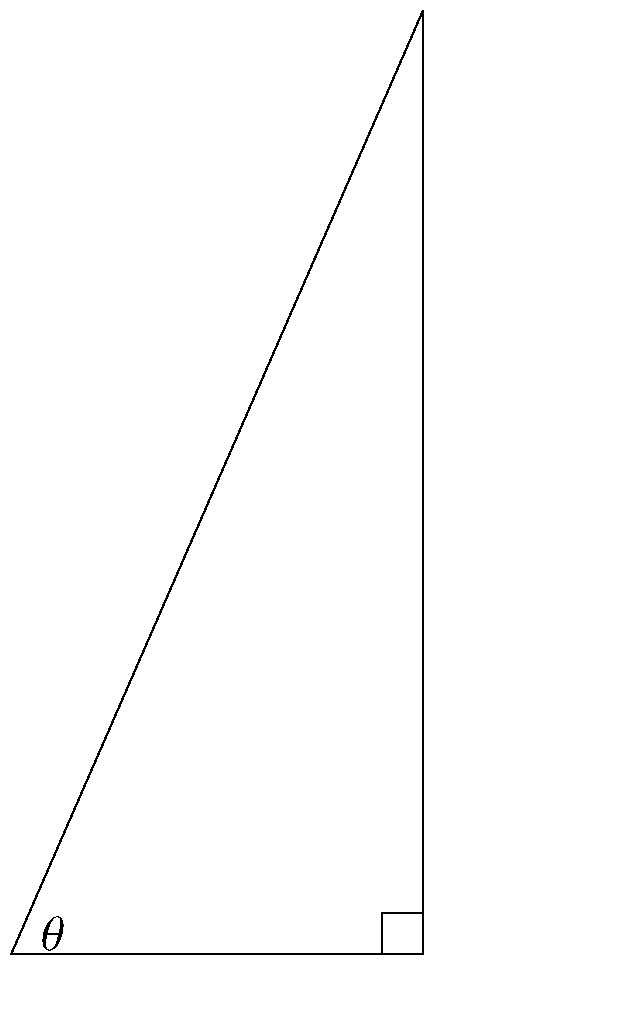
\includegraphics[height=6cm]{trigonometry/pictures/app-d-ex4a.pdf}%
}%
\only<handout:0| 2-3>{%
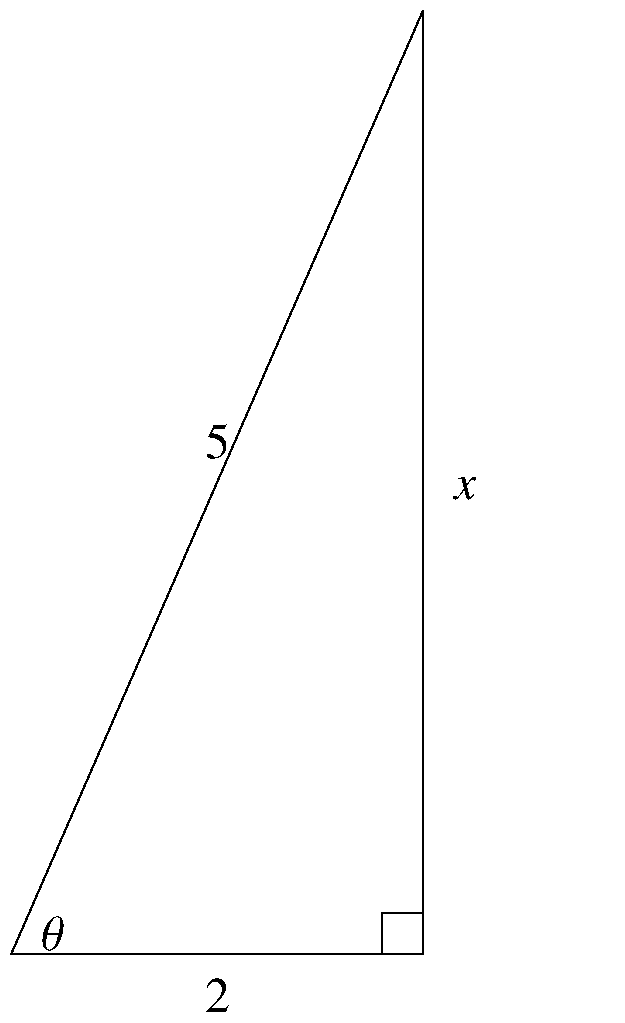
\includegraphics[height=6cm]{trigonometry/pictures/app-d-ex4b.pdf}%
}%
\only<4->{%
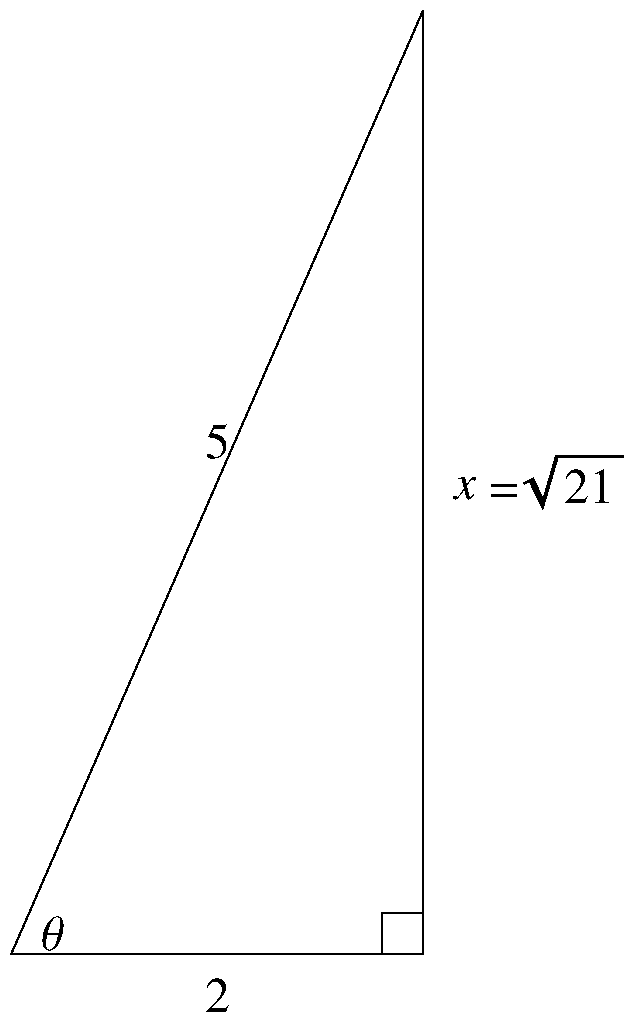
\includegraphics[height=6cm]{trigonometry/pictures/app-d-ex4c.pdf}%
}%
\column{.7\textwidth}
\begin{itemize}
\item<2->  Label the hypotenuse with length 5 and the adjacent side with length 2.
\item<3->  Pythagorean theorem: $x^2 +2^2 = 5^2$.
\item<4->  Therefore $x^2 = 21$, so $x = \sqrt{21}$.
\end{itemize}
\[
\begin{array}{cc}
\alert<handout:0| 5-6>{%
\sin \theta = %
\uncover<6->{%
\frac{\sqrt{21}}{5}%
}}&%
\alert<handout:0| 7-8>{%
\tan \theta = %
\uncover<8->{%
\frac{\sqrt{21}}{2}%
}}\\%
& \\
\alert<handout:0| 9-10>{%
\csc \theta = %
\uncover<10->{%
\frac{5}{\sqrt{21}}%
}}&%
\alert<handout:0| 11-12>{%
\sec \theta = %
\uncover<12->{%
\frac{5}{2}%
}}\\%
& \\
\alert<handout:0| 13-14>{%
\cot \theta = %
\uncover<14->{%
\frac{2}{\sqrt{21}}%
}}&%
\end{array}
\]
\end{columns}
\end{example}
\end{frame}
% end module trig-functions-example2
